%Dave's handout 1.7 intro 2nd derivatives
%Dave's handout 2.2 2nd derivative rule
\vspace{-0.25 in}
\begin{framed}
\subsection*{Objectives}
\begin{itemize}
    \item Define absolute extrema and local extrema.
    \item Use first derivative test and second derivative test to find local extrema.
    \item Locate absolute extrema over a closed interval.
\end{itemize}

%%%Reading Assignment%%%
\subsection*{Suggested Reading:}
\begin{itemize}
\item \cite{Calaway}\footnotemark[1]
   \begin{itemize}
        \item \emph{Section 2.7 Optimization}
    \end{itemize}
\item \cite{openstax}\footnotemark[2]
    \begin{itemize}
        \item \emph{Section 4.3  Maxima and Minima}
        \item \emph{Section 4.5 Derivatives and teh Shape of a Graph}
    \end{itemize}
\item \cite{activeCalc}\footnotemark[3]
    \begin{itemize}
        \item \emph{Section 3.1 Using derivatives to identify extreme values}
    \end{itemize}
\end{itemize}
%\subsection*{Supplemental Materials:}
%%%Key Terms%%%
\subsection*{Key Terms and Concepts:} 

\begin{multicols}{2}
\begin{itemize}
    \item Critical Numbers
    \item Sign Chart
    \item First Derivative Test
    \item Local Maximum and Local Minimum
    \item A Closed Interval
    \item An Open Interval
    \item Absolute Maximum and Absolute Minimum
\end{itemize}
\end{multicols}
\end{framed}
\footnotetext[1]{Available free to download from \url{http://www.opentextbookstore.com/details.php?id=14} .}
\footnotetext[2]{Available free to download from \url{https://openstax.org/details/books/calculus-volume-1}.}
\footnotetext[3]{Available free to download from \url{https://activecalculus.org/single/frontmatter.html}.}

\newpage
%%%%%%%%%%START LESSON CONTENT%%%%%%%%%%%%%
%\noindent\makebox[\linewidth]{\rule{\textwidth}{0.8pt}}
\Opensolutionfile{ans}[ans8]
\Opensolutionfile{ansL}[ansL8]
%%%%%%%%%%%%%%%%Start First Topic%%%%%%%%%%%%%%%%%%%%%%%%%%%%%
\noindent Given a particular function, we are often interested in determining the largest and smallest values of the function. This information is important in creating accurate graphs. Finding the maximum and minimum values of a function also has practical significance because we can use this method to solve optimization problems, such as maximizing profit, minimizing the amount of material used in manufacturing an aluminum can, or finding the maximum height a rocket can reach. In this section, we look at how to use derivatives to find the largest and smallest values for a function.\\


\begin{tcolorbox}[title = {Global Extreme Points }]
\begin{itemize}[leftmargin=*]
\item A \textbf{global maximum} point is the point at which the largest value of the function occurs.Formally, we say
    \begin{itemize}
        \item $f$ has a \textbf{global maximum} at $c$ if $f(c)\ge f(x)$ for all $x$ in the domain of $f$.
    \end{itemize}
\item A \textbf{global minimum} point is the point at which the smallest value of the function occurs. Formally, we say
    \begin{itemize}
        \item $f$ has a \textbf{global minimum} at $c$ if $f(c)\le f(x)$ for all $x$ in the domain of $f$.
    \end{itemize}
\end{itemize}
\end{tcolorbox}
\vspace{-0.5cm}
\subsubsection*{Notes:}
\begin{itemize}
    \item These points are also referred to as “absolute” maximum and minimum points.
    \item Every global extreme is also a local extreme but there are local extremes that are NOT global extremes.
\end{itemize}
\vspace{-0.5cm}
\begin{figure}[h]
    \centering
    \caption{} 
    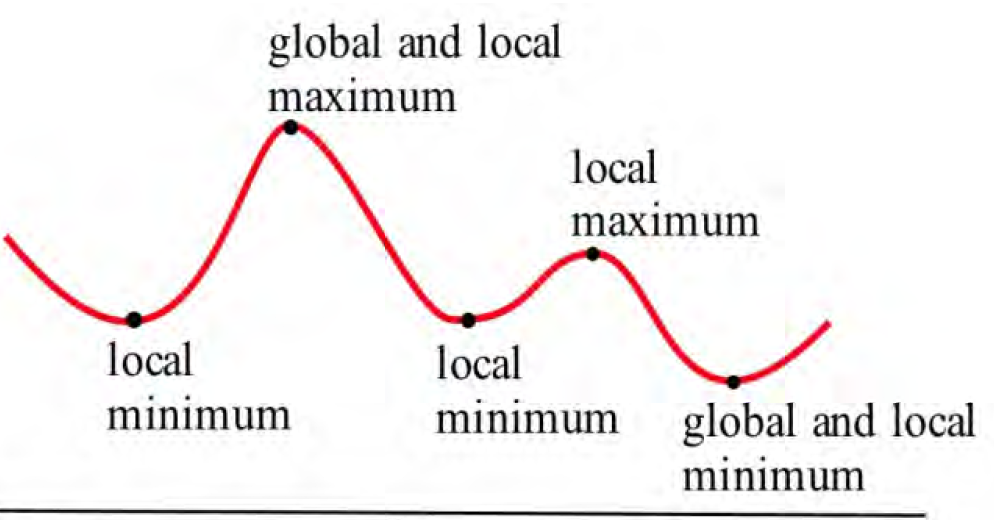
\includegraphics[scale=0.4]{images/optimization/globalVSlocalExtrema.png} 
    \label{fig:globalVSlocalExtrema}
\end{figure}

\begin{tcolorbox}[title={Steps For Locating Global Extrema Over A Closed Interval}]
Consider a continuous function $f$ defined over the closed interval $[a, b]$.
\begin{enumerate}
    \item Evaluate $f$ at the endpoints $x=a$ and $x=b$.
    \item Find all critical points of $f$ that lie over the interval $(a,b)$ and evaluate $f$ at those critical points.
    \item Compare all values found in (1) and (2). Since \underline{the global extrema must occur at endpoints or critical points}, the largest of these values is the global maximum of $f$ . The smallest of these values is the global minimum of $f$ .
\end{enumerate}
\end{tcolorbox}
\newpage
%%%Example: Calaway, Applied Calculus; section 2.7; Example 6%%%
\begin{example}
Given $f(x)=x^3-3x^2-9x+5$ for $-2\le x\le 6$, determine all \textbf{local extrema} using the \emph{First Derivative Test}. Follow the \emph{Five Steps for finding where $f$ is increasing/decreasing or any local extrema}. Then, use the steps described above to locate any \textbf{global extrema}.
    %%short answer
    \begin{sol}
    Local max of 10 at $x=-1$; local (and global) min of $-22$ at $x=3$; global max of $59$ when $x=6$.
    \end{sol}
    %%solution
    \begin{solL}
    Complete solution here.....
    
    \end{solL}
    
\end{example}
%\vspace*{\stretch{1}}
\newpage
\begin{tcolorbox}[title={Locating Global Extrema Over An Open Interval}]
\noindent If you are trying to find a global max or min on an open interval (or the whole real line), and there is more than one critical point, then you need to look at the graph to decide whether there is a global max or min. \underline{Be sure that all your critical points show in your graph}, and that you go a little beyond – that will tell you what you want to know.
\end{tcolorbox}
%%%Example: Dave's handout 2.3 Derivatives: Behavior and graph of a function%%%
\begin{example}\label{1stDervTest}
For each of the following functions, determine all \textbf{local extrema} using the \emph{First Derivative Test}. Follow the \emph{Five Steps for finding where $f$ is increasing/decreasing or any local extrema}. Then, use the given graph of each function to help determine any \textbf{global extrema}.
\renewcommand{\labelenumi}{(\alph{enumi})}
\begin{enumerate}[leftmargin=*]
    \item $f(x)=\displaystyle\frac{1}{3}x^3-\frac{5}{2}x^2+4x$. %%OpenStax; 4.3 Maxima and Minima; ex.4.12a
    \begin{figure}[h!]
        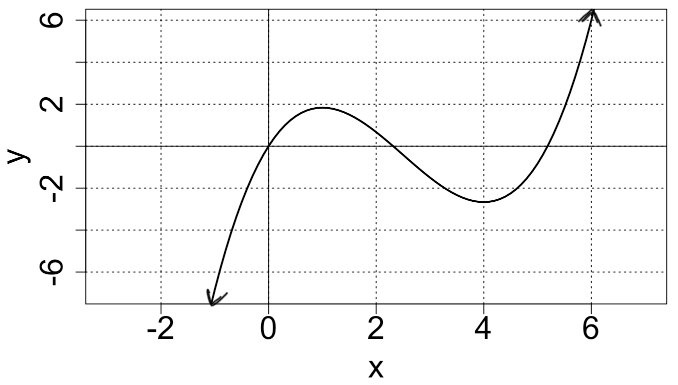
\includegraphics[width=0.45\textwidth,inner]{images/optimization/exampleGraph2.png}
        \label{fig:exampleGraph2}
    \end{figure}
 \vspace*{\stretch{2}}
    \item $f(x)=(x^2-1)^3$. %%OpenStax; 4.3 Maxima and Minima; ex.4.12b
    \begin{figure}[h!]
        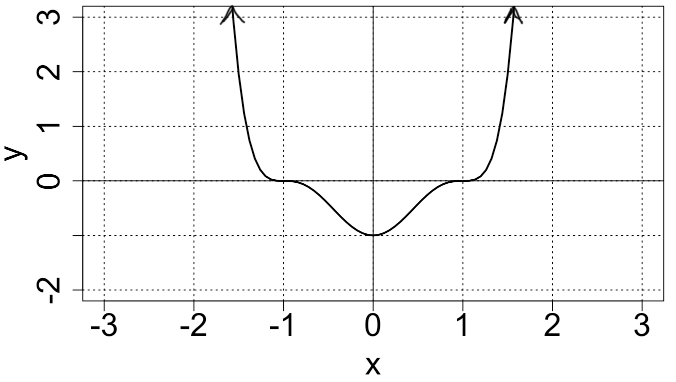
\includegraphics[width=0.45\textwidth,inner]{images/optimization/exampleGraph3.png}
        \label{fig:exampleGraph3}
    \end{figure}
    \vspace*{\stretch{1}}
    \newpage
    \item $f(x)=x+\displaystyle\frac{100}{x-1}$.  %%%Example: Dave's handout 2.3 Derivatives: Behavior and graph of a function%%%
    \begin{figure}[h!]
        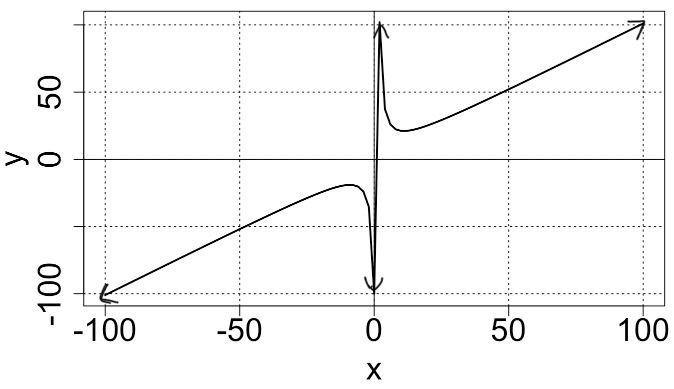
\includegraphics[width=0.45\textwidth,inner]{images/optimization/exampleGraph4.png}
        \label{fig:exampleGraph4}
    \end{figure}
     \vspace{1in}
    \item $f(x)=\displaystyle\frac{10}{x+2}$. %%%Example: Dave's handout 2.3 Derivatives:Behavior and graph of a function%%%
    \begin{figure}[h!]
        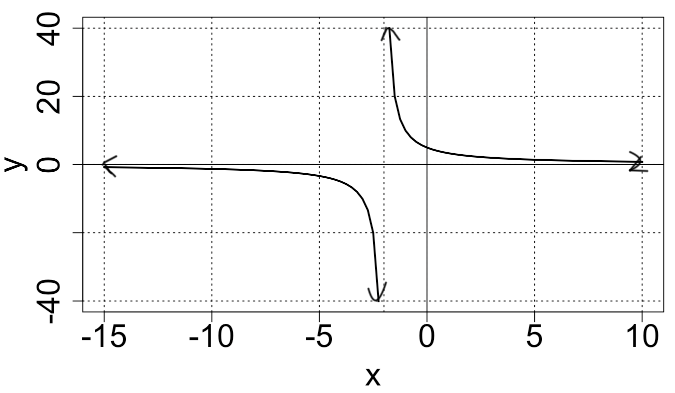
\includegraphics[width=0.45\textwidth,inner]{images/optimization/exampleGraph5.png}
        \label{fig:exampleGraph5}
    \end{figure}
     \vspace{1in}
\end{enumerate}
    %%short answer
    
    \begin{sol}
    (a) local max at $x=1$;local min at $x=4$;no global extrema. (b) only local (and global) minimum at $x=0$. (c) local max at $x=-9$; local min at $x=11$; no global extrema. (d) no extrema.
    \end{sol}
    %%solution
    \begin{solL}
    Complete solution here.....
    
    \end{solL}
    
\end{example}


%\vspace*{\stretch{1}}

%%%%%%%%%%%%End Examples%%%%%%%%%%%%%%%%%%
%%%%%%%%%%%%%%%End Topic%%%%%%%%%%%%%%%%%%



%%%%%%%%%%%%%%%End Lesson%%%%%%%%%%%%%%%%%%
\Closesolutionfile{ans}
\Closesolutionfile{ansL}

%%%Short Answers to Examples%%%
\vspace*{\fill}
\subsection*{Short Answers to Examples}
%\vspace{-0.25cm}

\input{ans8}



